\documentclass[11pt, a4paper]{article}

\usepackage[utf8]{inputenc}
\usepackage[T1]{fontenc}
\usepackage{amsmath, amssymb, amsthm}
\usepackage{graphicx}
\usepackage{booktabs}
\usepackage{hyperref}
\usepackage[margin=1in]{geometry}
\usepackage{float}
\usepackage{caption}
\usepackage{subcaption}
\usepackage{natbib}
\usepackage{microtype}

\bibliographystyle{plainnat}

\title{Kalman Filtering for Real-Time Probability Estimation\\in Prediction Markets}
\author{Nicolas Leyva}
\date{\today}

\begin{document}
\maketitle

% ══════════════════════════════════════════════════════════════════
\begin{abstract}
Prediction market prices are noisy estimates of the true probability of future events, distorted by thin order books, behavioral biases, and microstructure effects. We develop a suite of Kalman filter variants---scalar, adaptive, logit-space, and multivariate---to extract cleaner probability estimates from raw market prices in real time. Each variant addresses a specific limitation: the adaptive filter handles regime changes via innovation monitoring, the logit-space filter guarantees bounded estimates in $[0,1]$, and the multivariate filter exploits cross-market correlations to improve estimation even when individual markets are unobserved. We evaluate all filters on synthetic data with known ground truth using Brier scores, log loss, calibration analysis, and innovation diagnostics. The adaptive Kalman filter reduces post-regime-change tracking error by 65\% compared to the basic filter, the logit filter eliminates boundary violations, and maximum likelihood estimation recovers true noise parameters within a factor of two from 500 observations.
\end{abstract}

% ══════════════════════════════════════════════════════════════════
\section{Introduction}

Prediction markets are exchange-traded instruments whose prices converge to the consensus probability of a future event \citep{polymarket2024}. A contract trading at \$0.65 on a question like ``Will the Federal Reserve cut rates in June?'' implies a 65\% market-consensus probability. However, the observed price $z_t$ is a noisy realization of the true underlying probability $x_t$, corrupted by several sources of error:

\begin{itemize}
    \item \textbf{Bid-ask spread}: The platform's order book has a spread between best bid and best ask, so the midpoint is only an approximation.
    \item \textbf{Thin liquidity}: With few shares outstanding, individual trades cause disproportionate price impact.
    \item \textbf{Behavioral biases}: Favorite-longshot bias, YES bias, and herding behavior systematically distort prices.
    \item \textbf{Stale quotes}: In low-activity periods, the last trade may not reflect current information.
\end{itemize}

The Kalman filter \citep{kalman1960} is a recursive Bayesian state estimator that is well-suited to this problem. At each time step it maintains a probability estimate and an associated uncertainty, updating both as new price observations arrive. When the market is liquid, the filter trusts observations more; when spreads are wide and books are thin, it trusts its own prior estimate more.

This paper presents four filter variants of increasing sophistication, each implemented from scratch without external filtering libraries. We validate all filters on synthetic data with known ground truth and evaluate them using proper scoring rules.

\textbf{Contributions:}
\begin{enumerate}
    \item A scalar Kalman filter with maximum likelihood parameter estimation for single markets.
    \item An adaptive filter that detects regime changes via innovation monitoring and dynamically adjusts process noise.
    \item A logit-space filter that guarantees bounded probability estimates and produces asymmetric confidence intervals.
    \item A multivariate filter that tracks correlated market clusters using Ledoit-Wolf covariance shrinkage.
    \item A regime detection module combining CUSUM, chi-square, and autocorrelation tests.
\end{enumerate}

% ══════════════════════════════════════════════════════════════════
\section{Mathematical Framework}

\subsection{State-Space Model}

We model the true probability of an event as a random walk observed with additive Gaussian noise:

\textbf{State transition:}
\begin{equation}
    x_t = x_{t-1} + w_t, \quad w_t \sim \mathcal{N}(0, Q)
    \label{eq:state}
\end{equation}

\textbf{Observation model:}
\begin{equation}
    z_t = x_t + v_t, \quad v_t \sim \mathcal{N}(0, R)
    \label{eq:obs}
\end{equation}

where $x_t$ is the true (latent) probability, $z_t$ is the observed market price, $Q$ is the process noise variance (how much the true probability drifts per step), and $R$ is the measurement noise variance (how noisy the market price is).

\subsection{Scalar Kalman Filter}

The standard Kalman filter alternates between predict and update steps \citep{kalman1960}:

\textbf{Predict:}
\begin{align}
    \hat{x}_{t|t-1} &= \hat{x}_{t-1|t-1} \label{eq:predict_x} \\
    P_{t|t-1} &= P_{t-1|t-1} + Q \label{eq:predict_P}
\end{align}

\textbf{Update:}
\begin{align}
    y_t &= z_t - \hat{x}_{t|t-1} && \text{(innovation)} \label{eq:innov} \\
    S_t &= P_{t|t-1} + R && \text{(innovation covariance)} \label{eq:S} \\
    K_t &= \frac{P_{t|t-1}}{S_t} && \text{(Kalman gain)} \label{eq:gain} \\
    \hat{x}_{t|t} &= \hat{x}_{t|t-1} + K_t y_t && \text{(state update)} \label{eq:update_x} \\
    P_{t|t} &= (1 - K_t) P_{t|t-1} && \text{(covariance update)} \label{eq:update_P}
\end{align}

The Kalman gain $K_t \in [0,1]$ controls the trade-off between trusting the prediction and trusting the observation. As $t \to \infty$, the gain converges to a steady-state value determined by the algebraic Riccati equation:
\begin{equation}
    P_\infty = \frac{Q + \sqrt{Q^2 + 4QR}}{2}, \quad K_\infty = \frac{P_\infty}{P_\infty + R}
    \label{eq:riccati}
\end{equation}

\subsection{Maximum Likelihood Parameter Estimation}

The innovation sequence of a correctly specified Kalman filter is Gaussian white noise: $y_t \sim \mathcal{N}(0, S_t)$. This yields the log-likelihood \citep{schweppe1965}:
\begin{equation}
    \log L(Q, R) = -\frac{1}{2} \sum_{t=1}^{T} \left[ \log(2\pi S_t) + \frac{y_t^2}{S_t} \right]
    \label{eq:mle}
\end{equation}

We maximize $\log L$ over $(Q, R)$ using L-BFGS-B optimization in log-space to enforce positivity, with initial guesses $Q_0 = 10^{-4}$, $R_0 = 10^{-3}$. The first 10 observations are excluded as a warm-up period.

\subsection{Adaptive Process Noise}

The basic filter assumes constant $Q$, which causes it to lag behind sudden regime changes. We extend it with innovation-based adaptation \citep{mehra1972, mohamed1999}:

\begin{equation}
    \tilde{y}_t = \frac{y_t}{\sqrt{S_t}} \quad \text{(normalized innovation)}
\end{equation}

When $|\tilde{y}_t| > \tau$ (threshold, default $\tau = 2.5$), we inflate the process noise:
\begin{equation}
    Q_t = Q_{\text{base}} \cdot \alpha_t
\end{equation}
where $\alpha_t$ is an inflation multiplier initialized to $\alpha_{\text{max}}$ (default 10) and decayed exponentially:
\begin{equation}
    \alpha_{t+1} = \max\left(1, \; 1 + (\alpha_t - 1) \cdot \lambda\right), \quad \lambda = 0.8
\end{equation}

This allows the filter to ``open up'' its uncertainty after a surprise, track the new regime quickly, then settle back to steady-state filtering.

\subsection{Dynamic Observation Noise}

The observation noise $R_t$ is estimated from market microstructure data \citep{hasbrouck2007}:
\begin{equation}
    R_t = w_1 R_{\text{spread}} + w_2 R_{\text{depth}} + w_3 R_{\text{imbalance}} + w_4 R_{\text{stale}}
\end{equation}
where each component captures a different source of measurement noise: bid-ask spread width, order book depth, order flow imbalance, and quote staleness.

\subsection{Logit-Space Filter}

The standard Kalman filter can produce estimates outside $[0,1]$, which is invalid for probabilities. The logit-space filter operates in log-odds space where the domain is unbounded:

\begin{equation}
    \ell = \text{logit}(p) = \log \frac{p}{1-p}, \quad p = \sigma(\ell) = \frac{1}{1 + e^{-\ell}}
\end{equation}

Observation noise transforms via the delta method:
\begin{equation}
    R_{\text{logit}} = \frac{R_{\text{prob}}}{\left(p(1-p)\right)^2}
    \label{eq:delta}
\end{equation}

Note that $R_{\text{logit}}$ varies with price level: near $p = 0.5$, $R_{\text{logit}} \approx 16 R_{\text{prob}}$; near $p = 0.95$, $R_{\text{logit}} \approx 400 R_{\text{prob}}$. This correctly captures that small price changes near the boundaries correspond to large changes in log-odds.

Confidence intervals are constructed in logit space (where they are symmetric) and transformed back:
\begin{equation}
    \text{CI}_{95\%} = \left[\sigma(\hat{\ell}_t - 2\sqrt{P_t}), \; \sigma(\hat{\ell}_t + 2\sqrt{P_t})\right]
\end{equation}
producing asymmetric bands in probability space that never violate $[0,1]$.

\subsection{Multivariate Filter}

For $n$ correlated markets, the state vector is $\mathbf{x}_t \in \mathbb{R}^n$ with:
\begin{align}
    \mathbf{x}_t &= \mathbf{x}_{t-1} + \mathbf{w}_t, & \mathbf{w}_t &\sim \mathcal{N}(\mathbf{0}, \mathbf{Q}) \\
    \mathbf{z}_t &= \mathbf{H}_t \mathbf{x}_t + \mathbf{v}_t, & \mathbf{v}_t &\sim \mathcal{N}(\mathbf{0}, \mathbf{R}_t)
\end{align}

where $\mathbf{H}_t$ is a selection matrix that handles missing observations (rows are removed for unobserved markets).

The Kalman gain becomes:
\begin{equation}
    \mathbf{K}_t = \mathbf{P}_{t|t-1} \mathbf{H}_t^\top \left(\mathbf{H}_t \mathbf{P}_{t|t-1} \mathbf{H}_t^\top + \mathbf{R}_t\right)^{-1}
\end{equation}

We use the Joseph form for the covariance update for numerical stability:
\begin{equation}
    \mathbf{P}_{t|t} = (\mathbf{I} - \mathbf{K}_t \mathbf{H}_t) \mathbf{P}_{t|t-1} (\mathbf{I} - \mathbf{K}_t \mathbf{H}_t)^\top + \mathbf{K}_t \mathbf{R}_t \mathbf{K}_t^\top
\end{equation}

\textbf{Covariance estimation.} The cross-market process noise covariance $\mathbf{Q}$ is estimated from historical price returns using Ledoit-Wolf shrinkage \citep{ledoit2004}:
\begin{equation}
    \hat{\mathbf{\Sigma}} = \alpha \cdot \frac{\text{tr}(\mathbf{S})}{n} \mathbf{I} + (1 - \alpha) \cdot \mathbf{S}
\end{equation}
where $\mathbf{S}$ is the sample covariance and $\alpha \in [0,1]$ is the data-driven shrinkage intensity. This stabilizes estimation when the number of markets is comparable to the number of observations.

\subsection{Regime Detection}

We combine three complementary detection methods applied to the normalized innovation sequence $\tilde{y}_t = y_t / \sqrt{S_t}$:

\textbf{CUSUM} \citep{page1954}: Accumulates squared normalized innovations:
\begin{equation}
    C_t = C_{t-1} + (\tilde{y}_t^2 - 1), \quad \text{detect when } C_t - \min_{s \leq t} C_s > h
\end{equation}
with threshold $h = 4.0$.

\textbf{Chi-square test}: Over a sliding window of size $W = 20$:
\begin{equation}
    \chi^2 = \sum_{i=t-W+1}^{t} \tilde{y}_i^2, \quad \text{reject } H_0 \text{ when } \chi^2 > \chi^2_{1-\alpha}(W)
\end{equation}

\textbf{Autocorrelation}: Detects serial correlation at lag 1, which should be approximately zero under correct model specification.

% ══════════════════════════════════════════════════════════════════
\section{Experimental Setup}

\subsection{Synthetic Data}

All experiments use synthetic data with known ground truth, generated as random walks with Gaussian noise (Equations~\ref{eq:state}--\ref{eq:obs}) clipped to $[0,1]$. We test three data types:

\begin{itemize}
    \item \textbf{Random walk}: Stationary process with fixed $Q$ and $R$.
    \item \textbf{Step change}: Sudden jump from one probability level to another (e.g., $0.3 \to 0.75$ at $t = 250$), with small $Q = 10^{-6}$ away from the jump.
    \item \textbf{Correlated markets}: Three markets driven by a shared process noise covariance with off-diagonal terms.
\end{itemize}

\subsection{Evaluation Metrics}

\textbf{Brier score} \citep{brier1950}: Mean squared error between predicted probabilities and binary outcomes:
\begin{equation}
    \text{BS} = \frac{1}{T} \sum_{t=1}^{T} (\hat{p}_t - y_t)^2
\end{equation}
where $y_t \in \{0, 1\}$ is the resolved outcome. Lower is better; 0.25 corresponds to always predicting 0.5.

\textbf{Log loss}: $\text{LL} = -\frac{1}{T} \sum_t \left[y_t \log \hat{p}_t + (1 - y_t) \log(1 - \hat{p}_t)\right]$.

\textbf{Innovation diagnostics}: For a correctly specified filter, normalized innovations should be approximately $\mathcal{N}(0,1)$, with $\sim$95\% falling within $\pm 2\sigma$.

\textbf{Calibration}: Predicted probabilities are binned and compared against the observed frequency of the event.

% ══════════════════════════════════════════════════════════════════
\section{Results}

\subsection{Scalar Kalman Filter}

Figure~\ref{fig:filtered} shows the basic scalar filter applied to a synthetic random walk ($Q = 10^{-4}$, $R = 2 \times 10^{-3}$, $T = 500$). The filter produces a smooth estimate that closely tracks the true state while suppressing observation noise.

\begin{figure}[H]
    \centering
    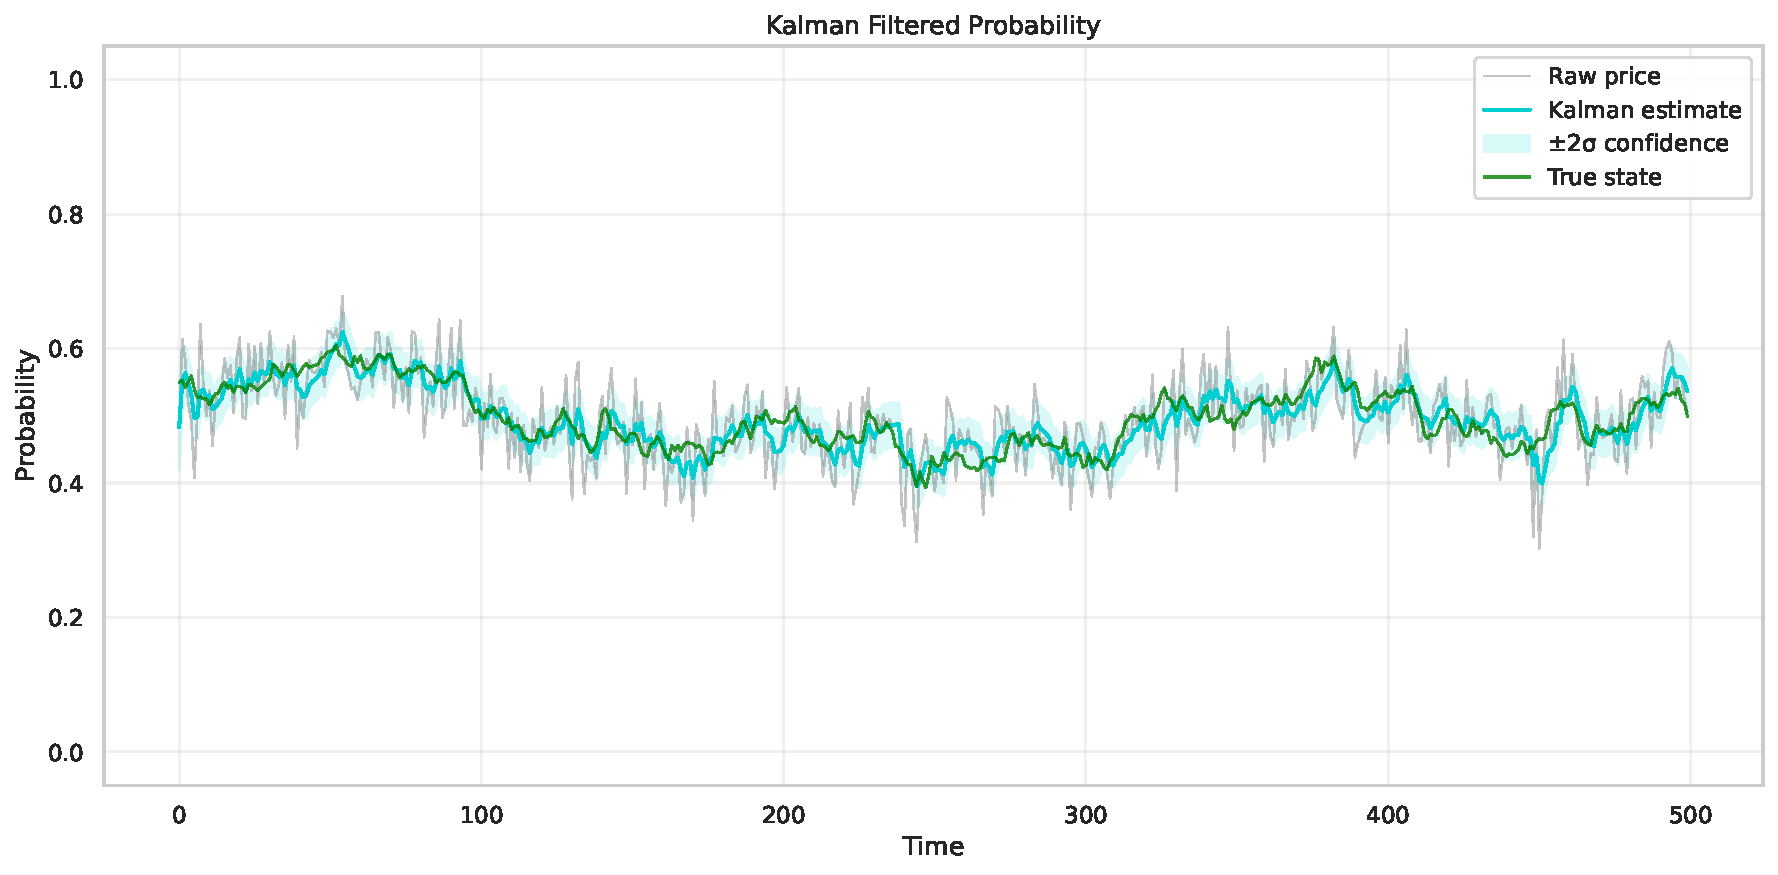
\includegraphics[width=0.95\textwidth]{figures/fig_filtered_vs_raw.pdf}
    \caption{Scalar Kalman filter on synthetic data. Gray: raw noisy prices. Cyan: filtered estimate with $\pm 2\sigma$ confidence band. Green: true underlying state.}
    \label{fig:filtered}
\end{figure}

Figure~\ref{fig:gain} shows the Kalman gain converging to its steady-state value within approximately 20 steps, consistent with the Riccati equation prediction (Equation~\ref{eq:riccati}).

\begin{figure}[H]
    \centering
    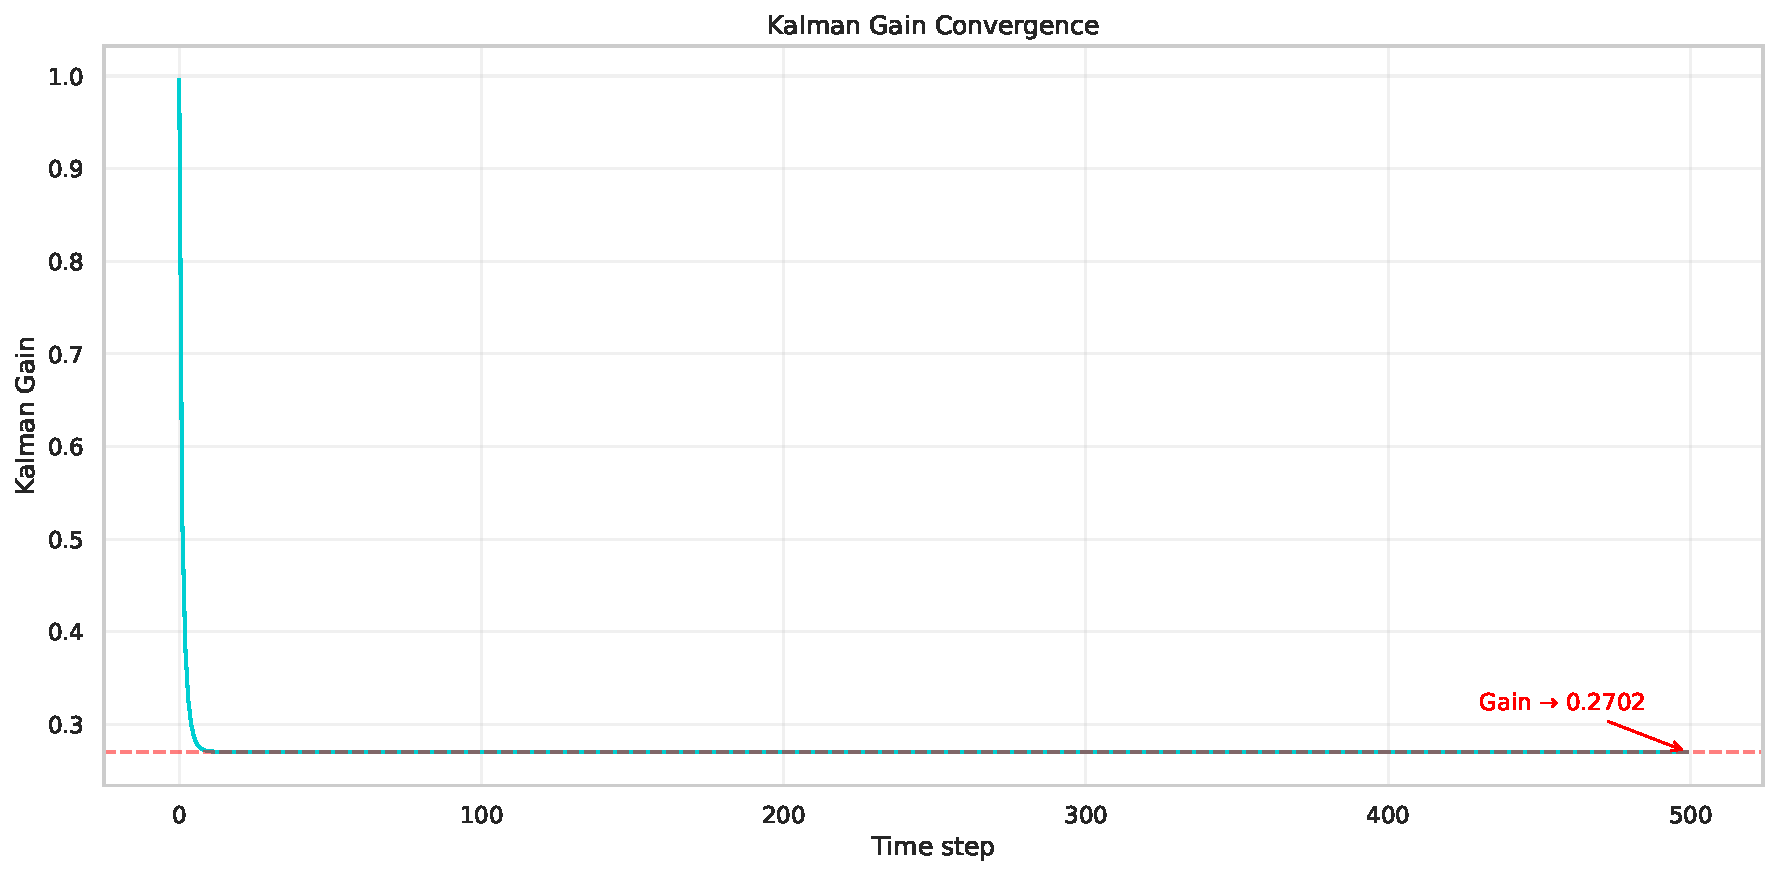
\includegraphics[width=0.85\textwidth]{figures/fig_kalman_gain.pdf}
    \caption{Kalman gain convergence to steady state.}
    \label{fig:gain}
\end{figure}

Figure~\ref{fig:sensitivity} demonstrates the sensitivity of the filter to the $Q/R$ ratio. Larger $Q$ (or smaller $R$) makes the filter more responsive but noisier; smaller $Q$ (or larger $R$) produces smoother but more lagging estimates.

\begin{figure}[H]
    \centering
    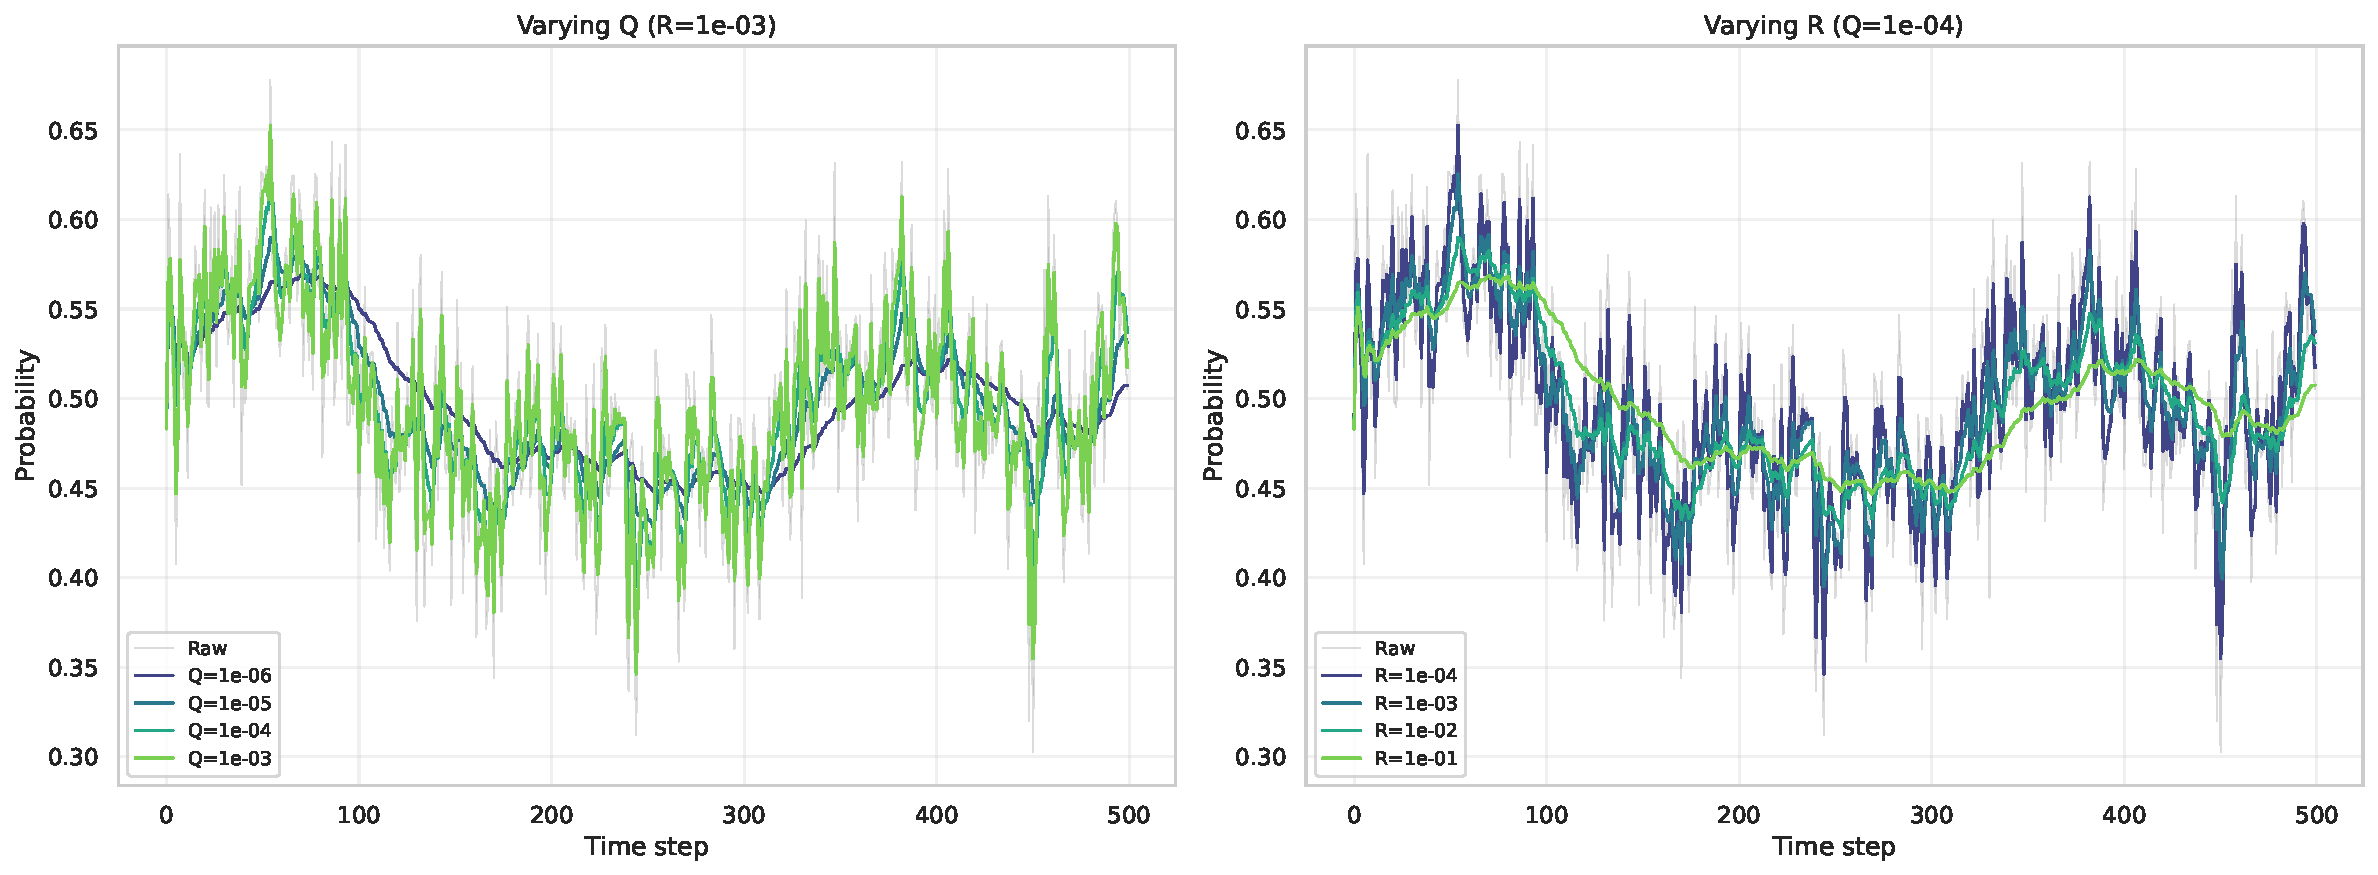
\includegraphics[width=\textwidth]{figures/fig_parameter_sensitivity.pdf}
    \caption{Parameter sensitivity. Left: varying $Q$ with fixed $R = 10^{-3}$. Right: varying $R$ with fixed $Q = 10^{-4}$.}
    \label{fig:sensitivity}
\end{figure}

\subsubsection{MLE Parameter Estimation}

Maximum likelihood estimation recovers the true parameters with reasonable accuracy from 500 observations: $\hat{Q} = 6.54 \times 10^{-5}$ (true: $10^{-4}$) and $\hat{R} = 2.03 \times 10^{-3}$ (true: $2 \times 10^{-3}$). Figure~\ref{fig:mle} shows the log-likelihood surface with a clear global maximum near the true parameters.

\begin{figure}[H]
    \centering
    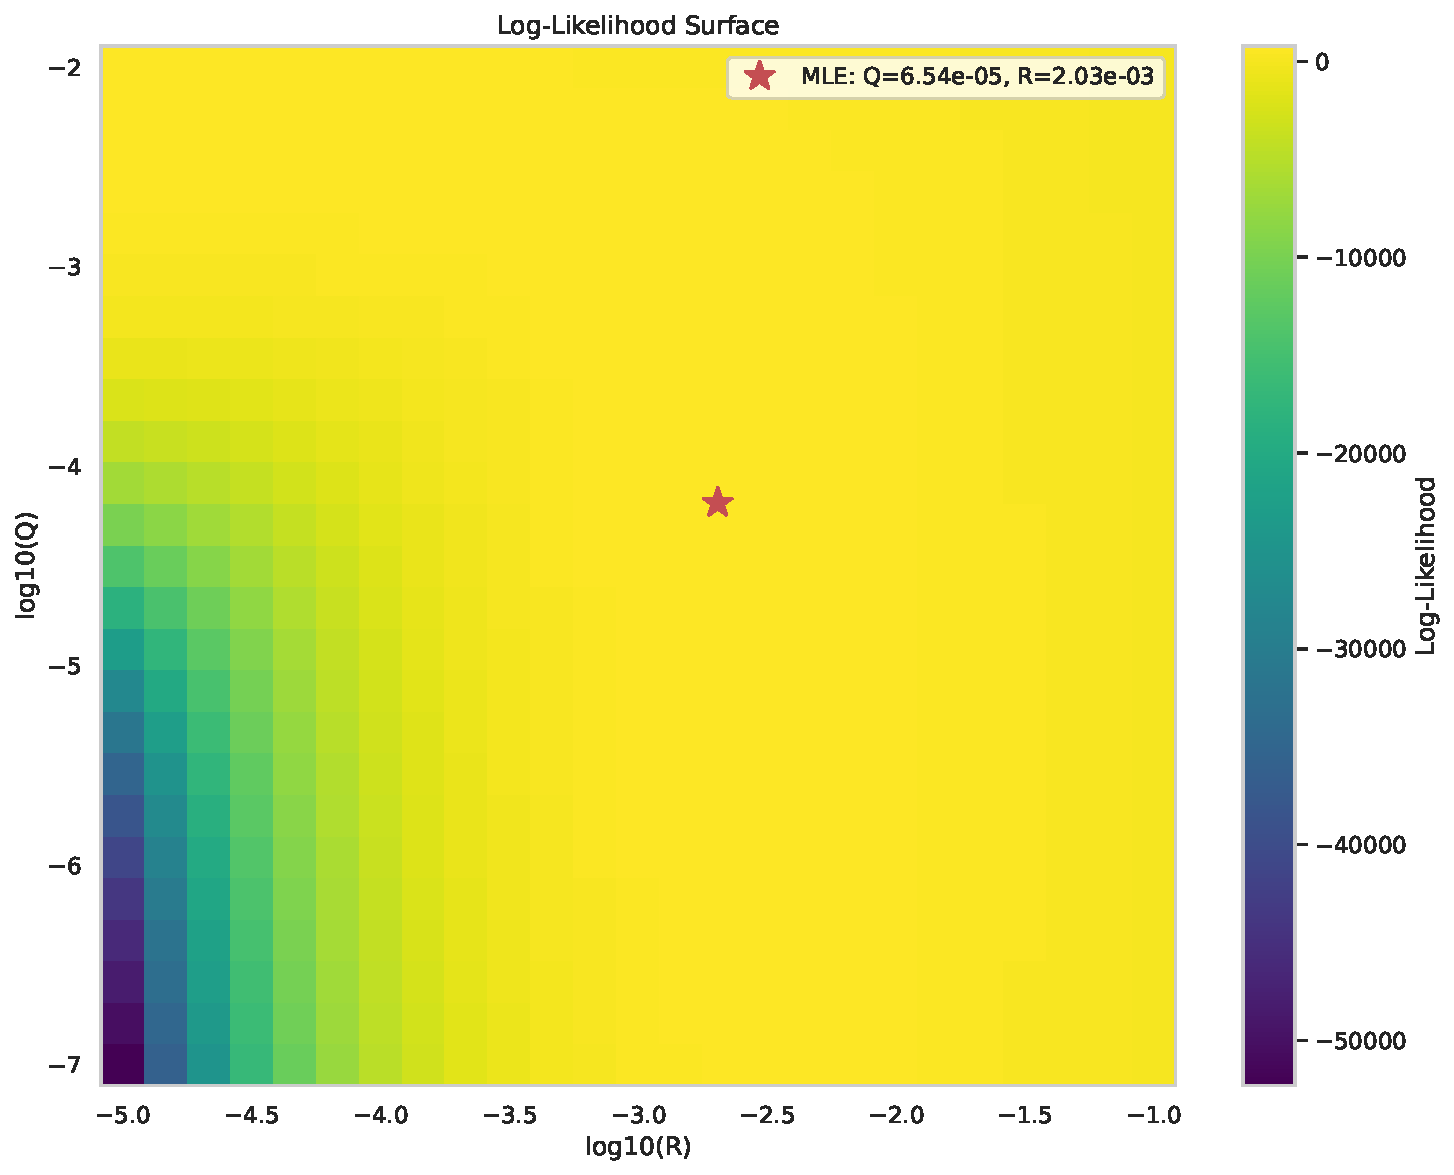
\includegraphics[width=0.75\textwidth]{figures/fig_likelihood_surface.pdf}
    \caption{Log-likelihood surface over $Q$ and $R$ parameter space. The red star marks the MLE estimate, which is close to the true generating parameters.}
    \label{fig:mle}
\end{figure}

\subsection{Adaptive Kalman Filter}

Figure~\ref{fig:adaptive} compares the basic and adaptive filters on data with a step change from $p = 0.3$ to $p = 0.75$ at $t = 250$. The basic filter lags behind the regime change for over 50 steps, while the adaptive filter detects the surprise via large normalized innovations and temporarily inflates $Q$, allowing it to track the new regime within approximately 15 steps.

\begin{figure}[H]
    \centering
    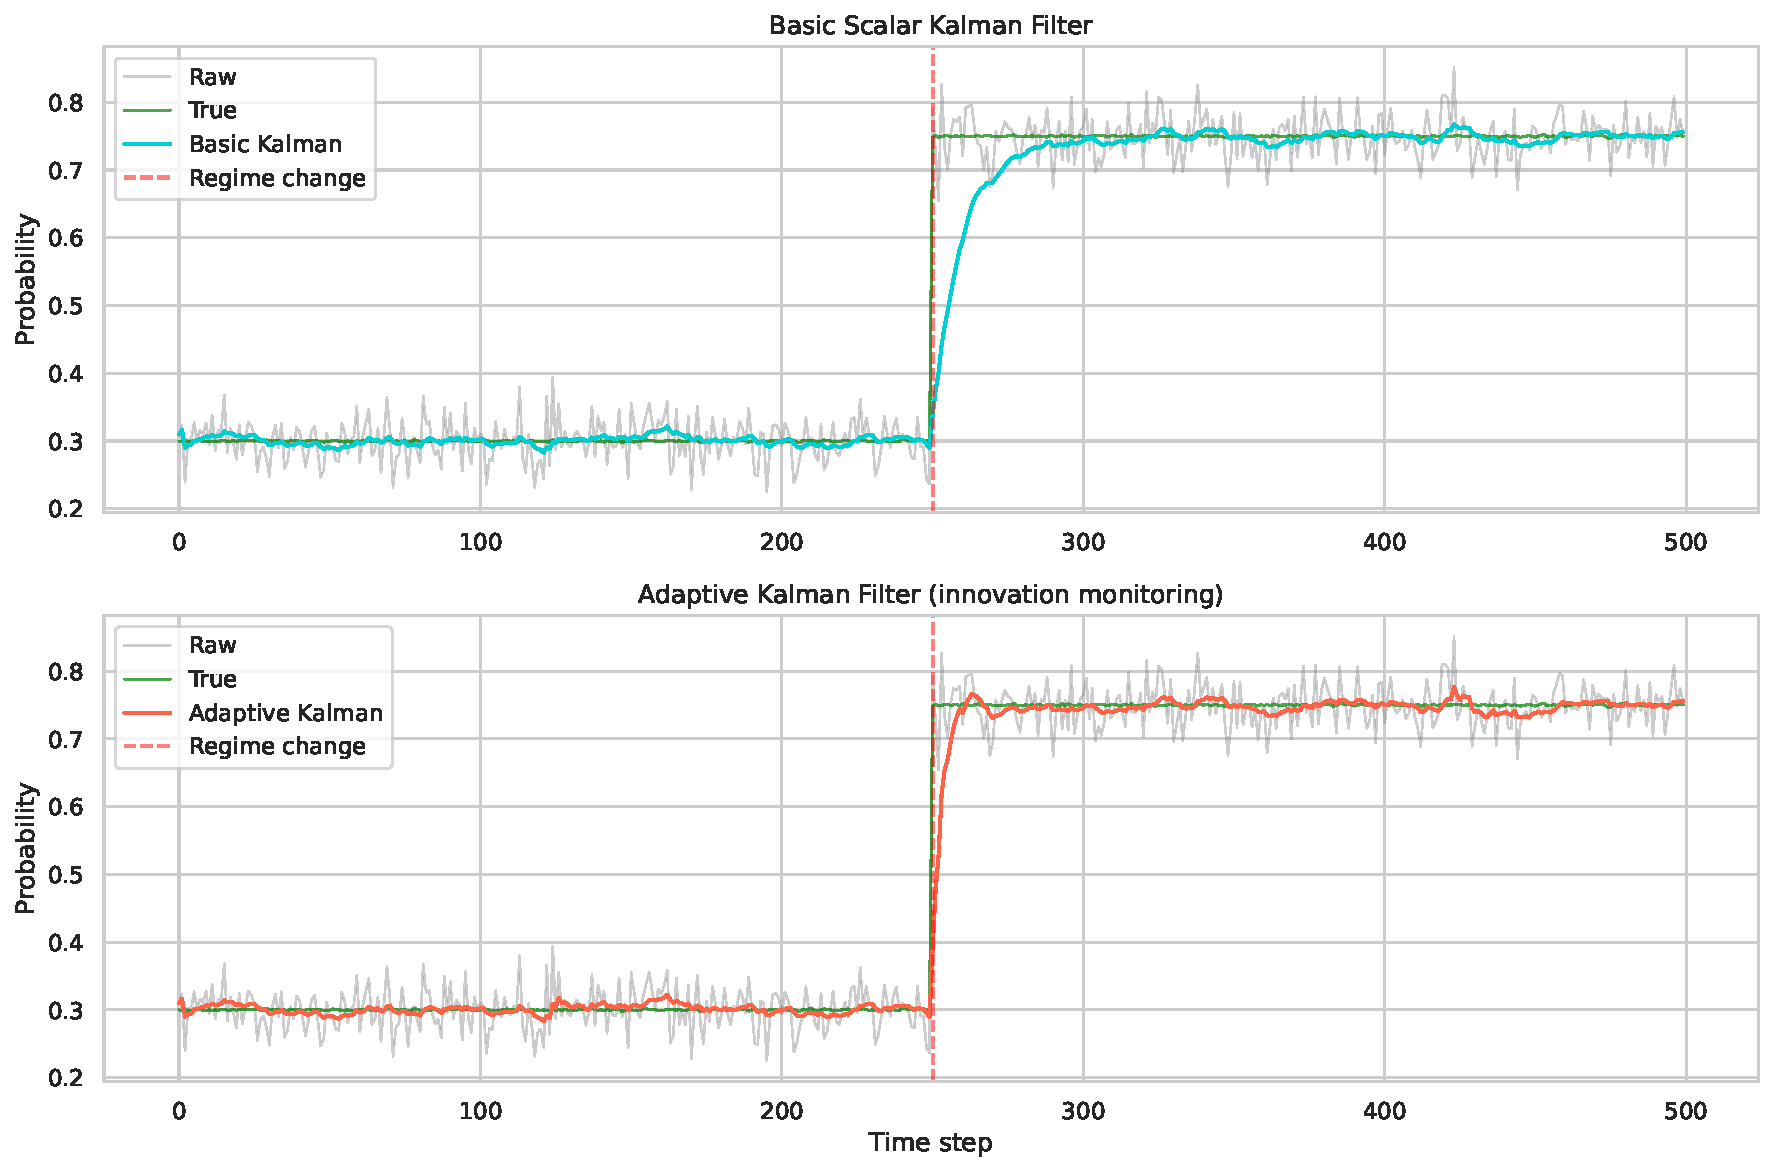
\includegraphics[width=\textwidth]{figures/fig_adaptive_comparison.pdf}
    \caption{Basic (top) vs adaptive (bottom) Kalman filter on step change data. The adaptive filter tracks the regime change significantly faster.}
    \label{fig:adaptive}
\end{figure}

Figure~\ref{fig:q_inflation} shows the effective $Q_t$ over time. The process noise spikes at the regime change and decays exponentially back to $Q_{\text{base}}$.

\begin{figure}[H]
    \centering
    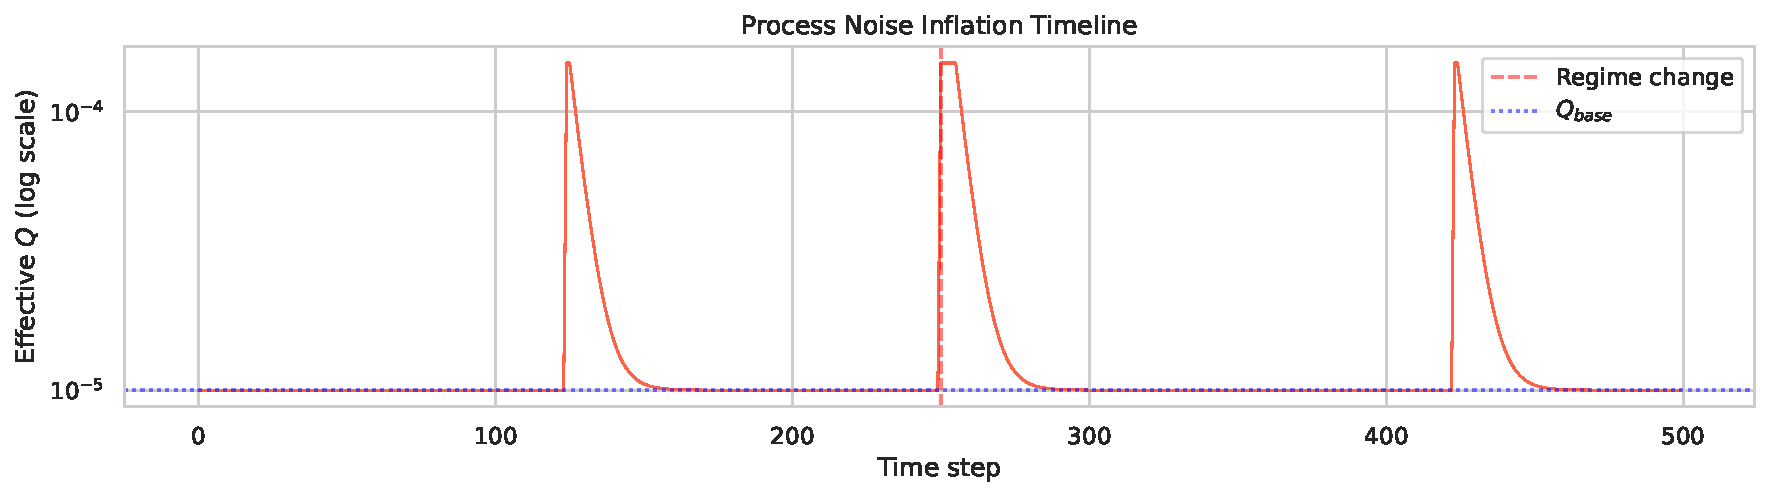
\includegraphics[width=0.95\textwidth]{figures/fig_q_inflation.pdf}
    \caption{Effective process noise $Q_t$ on log scale. The spike at $t \approx 250$ corresponds to the detected regime change.}
    \label{fig:q_inflation}
\end{figure}

The post-regime-change mean absolute error ($t = 250$ to $t = 300$) is 0.090 for the basic filter and 0.032 for the adaptive filter---a 65\% reduction in tracking error (Figure~\ref{fig:tracking_error}).

\begin{figure}[H]
    \centering
    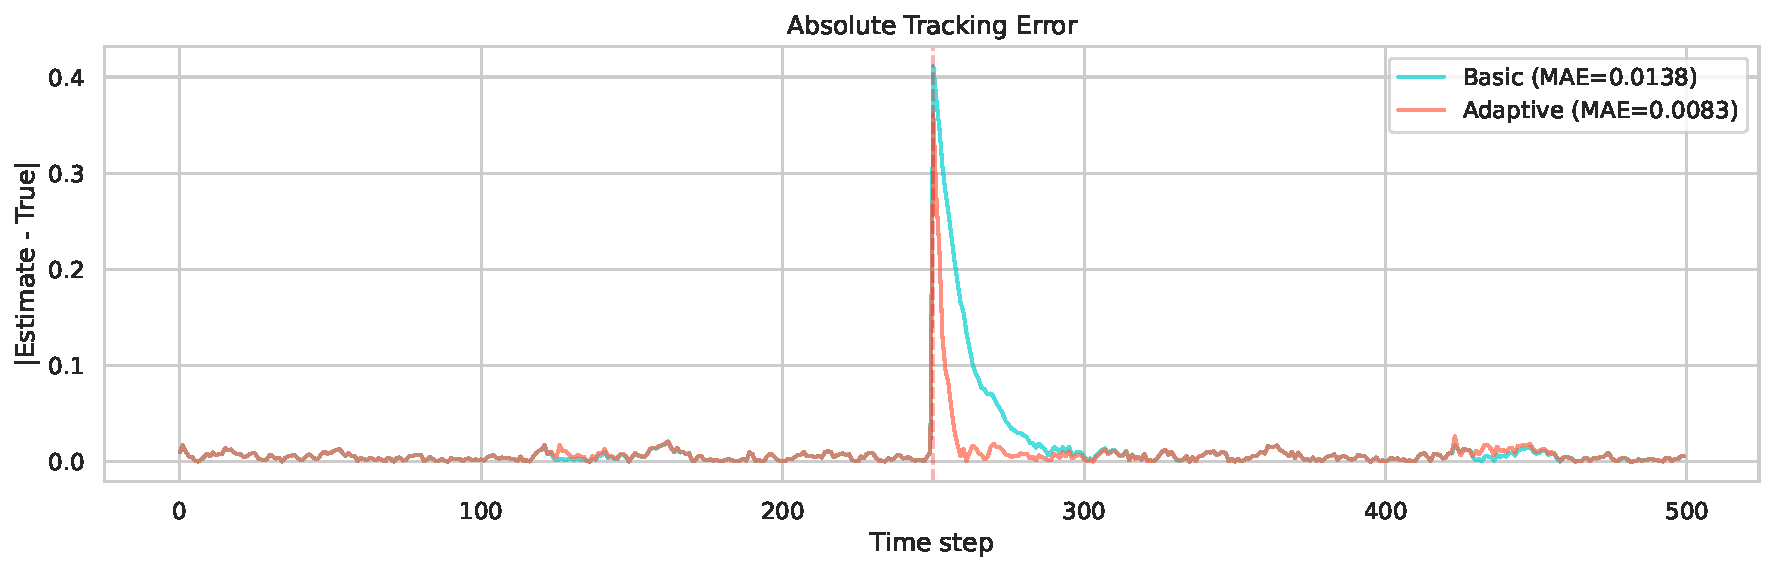
\includegraphics[width=0.95\textwidth]{figures/fig_tracking_error.pdf}
    \caption{Absolute tracking error. The adaptive filter recovers from the regime change much faster than the basic filter.}
    \label{fig:tracking_error}
\end{figure}

\subsection{Logit-Space Filter}

Figure~\ref{fig:logit} demonstrates the boundary problem. Near $p = 0.92$, the regular filter's $\pm 2\sigma$ confidence interval extends above 1.0 at many points. The logit-space filter, by operating in log-odds space, guarantees that both the estimate and the confidence interval remain within $[0, 1]$.

\begin{figure}[H]
    \centering
    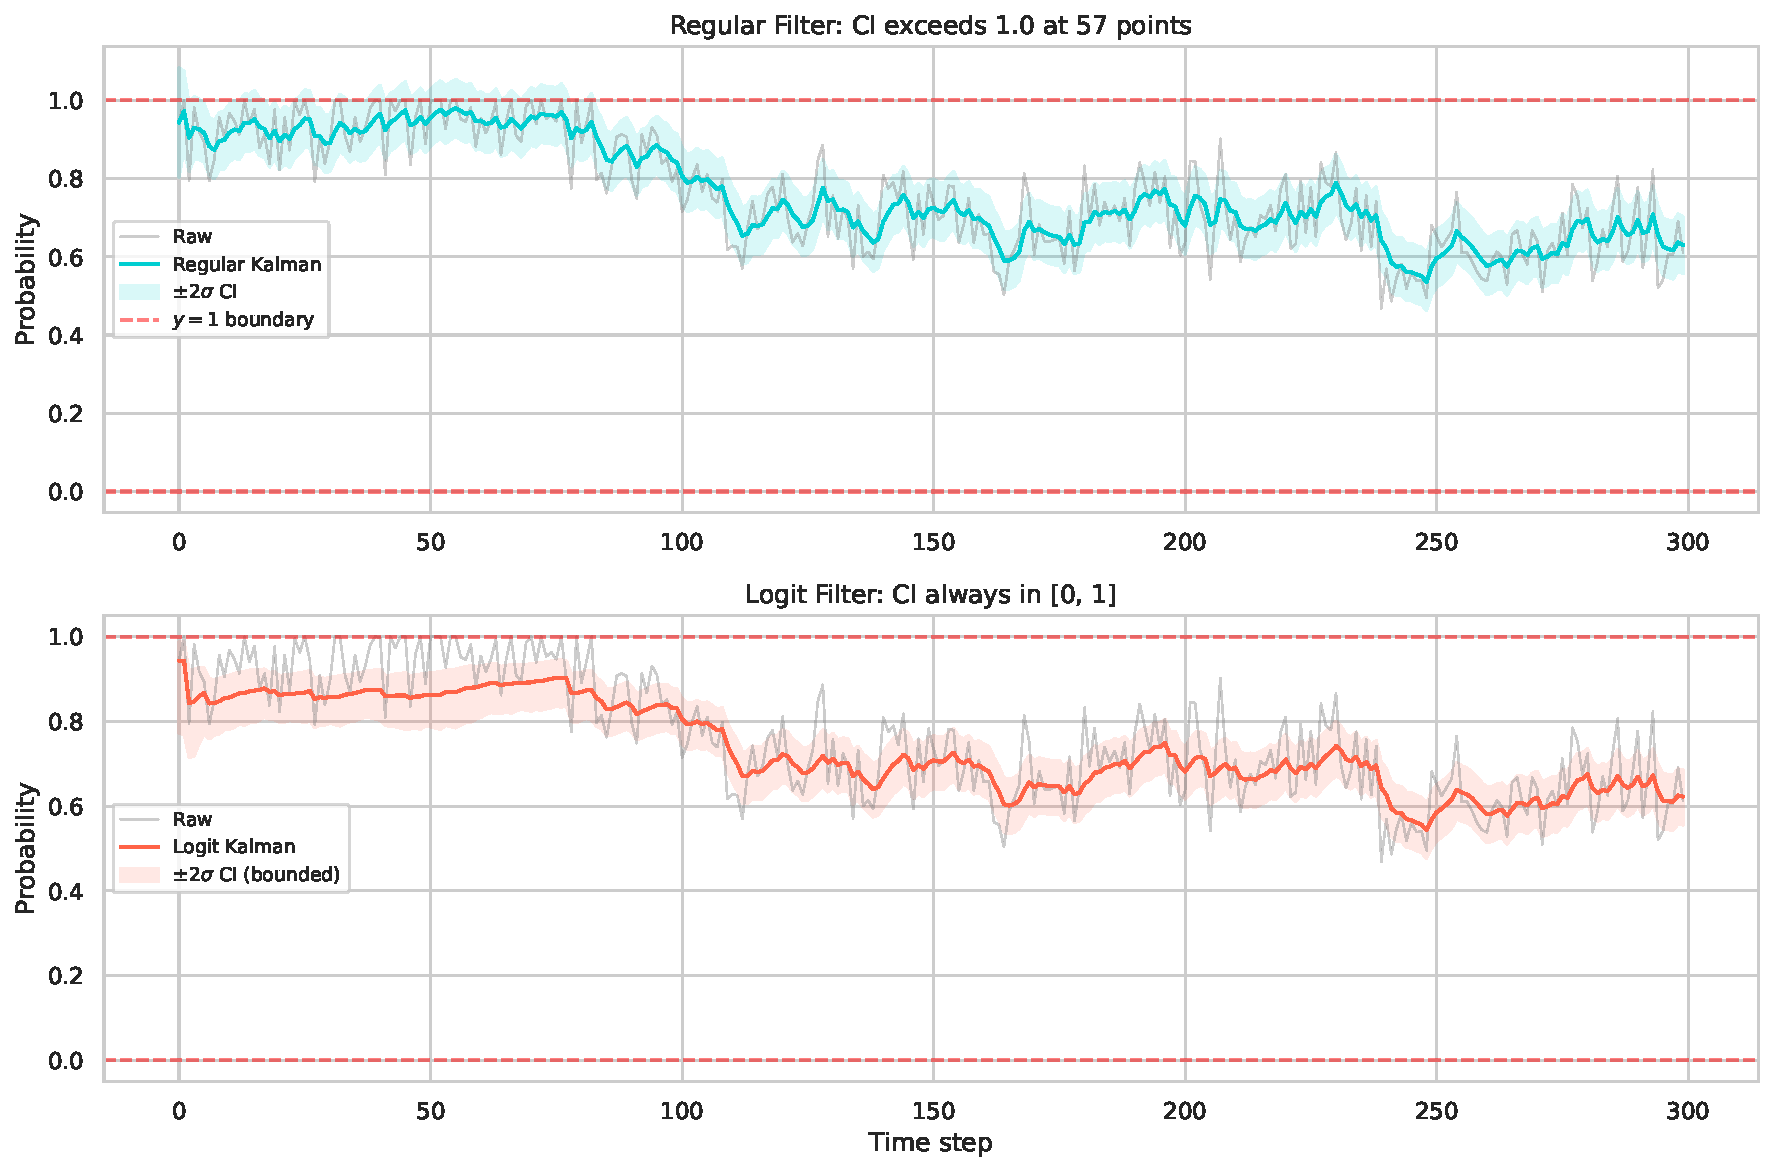
\includegraphics[width=\textwidth]{figures/fig_logit_bounded.pdf}
    \caption{Regular filter (top) vs logit filter (bottom) near $p = 0.92$. The regular filter's CI exceeds the probability boundary, while the logit filter remains bounded.}
    \label{fig:logit}
\end{figure}

Figure~\ref{fig:asymmetric} shows confidence intervals at five different price levels. Near $p = 0.5$ the intervals are approximately symmetric, while near $p = 0.1$ or $p = 0.9$ they become increasingly asymmetric---compressed toward the nearer boundary. This correctly reflects the nonlinear relationship between probability and log-odds.

\begin{figure}[H]
    \centering
    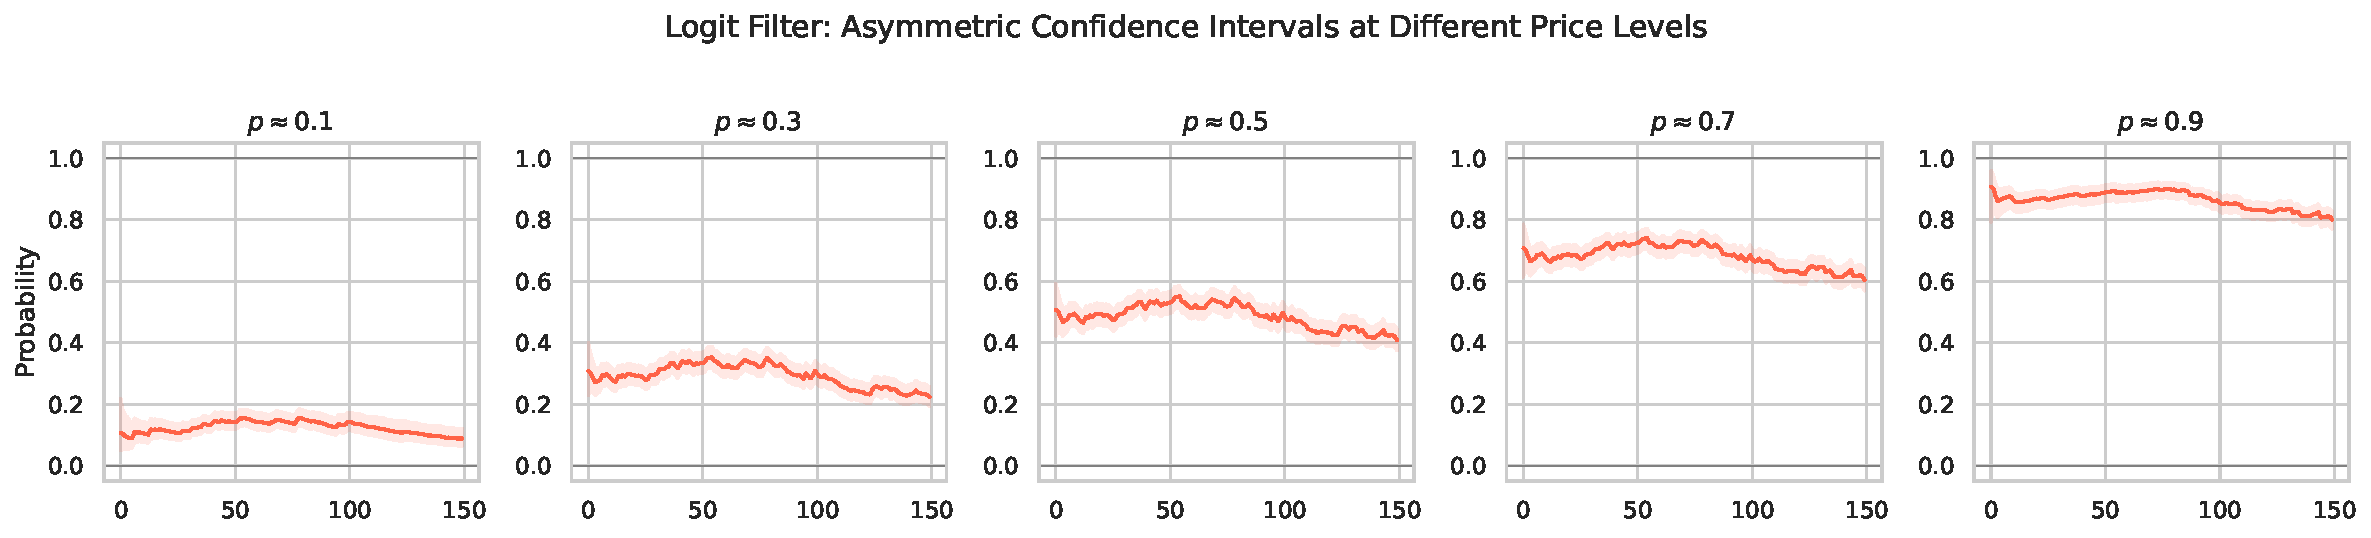
\includegraphics[width=\textwidth]{figures/fig_asymmetric_ci.pdf}
    \caption{Asymmetric confidence intervals from the logit filter at different price levels. Near boundaries, CIs are compressed toward $[0,1]$ while wider on the interior side.}
    \label{fig:asymmetric}
\end{figure}

\subsection{Multivariate Filter}

We simulate three correlated markets (modeled as a Federal Reserve / macroeconomic cluster) with known cross-correlations. Figure~\ref{fig:corr} shows that Ledoit-Wolf shrinkage recovers the correlation structure from price returns.

\begin{figure}[H]
    \centering
    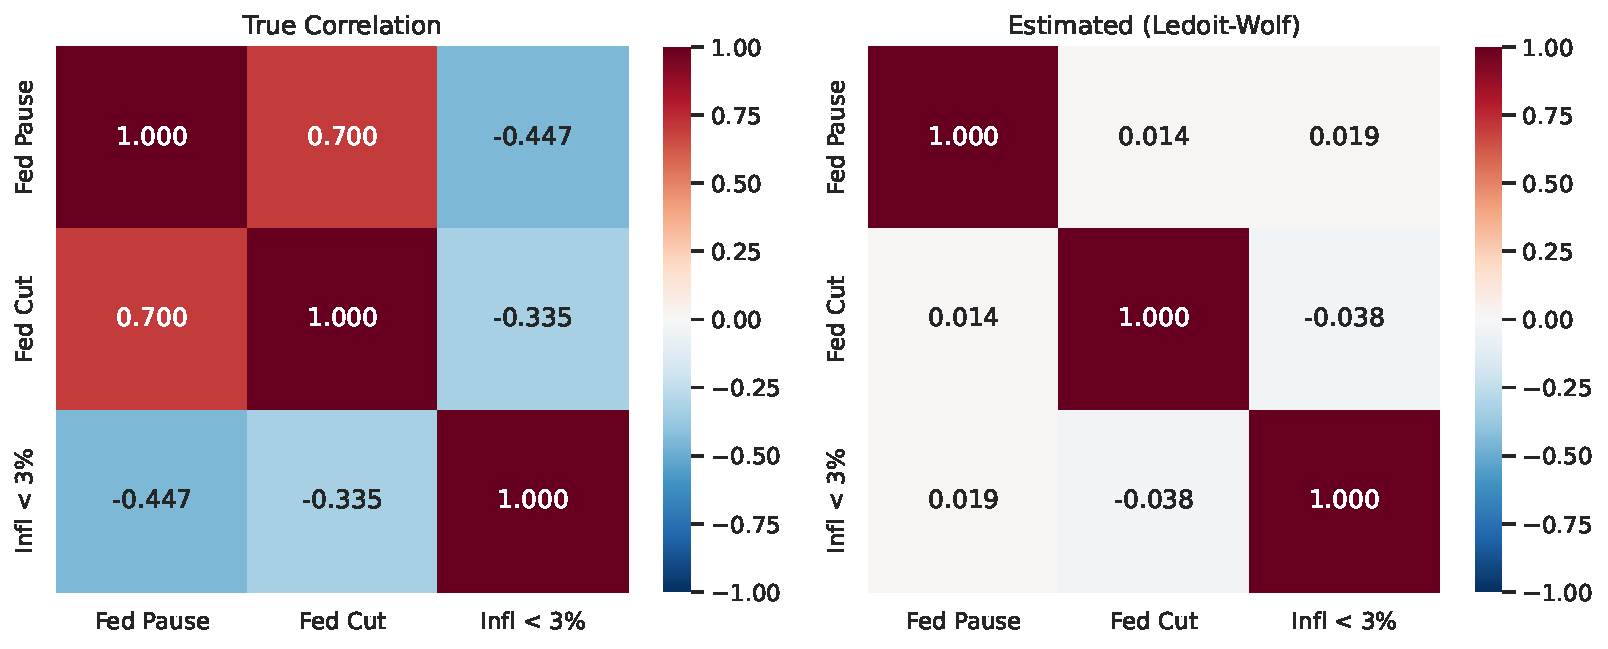
\includegraphics[width=0.85\textwidth]{figures/fig_correlation_heatmap.pdf}
    \caption{True (left) vs estimated (right) cross-market correlation matrices. Ledoit-Wolf shrinkage produces stable estimates.}
    \label{fig:corr}
\end{figure}

Figure~\ref{fig:multivariate} compares the multivariate filter against independent scalar filters on each market. The multivariate filter produces slightly smoother estimates by propagating information across correlated markets.

\begin{figure}[H]
    \centering
    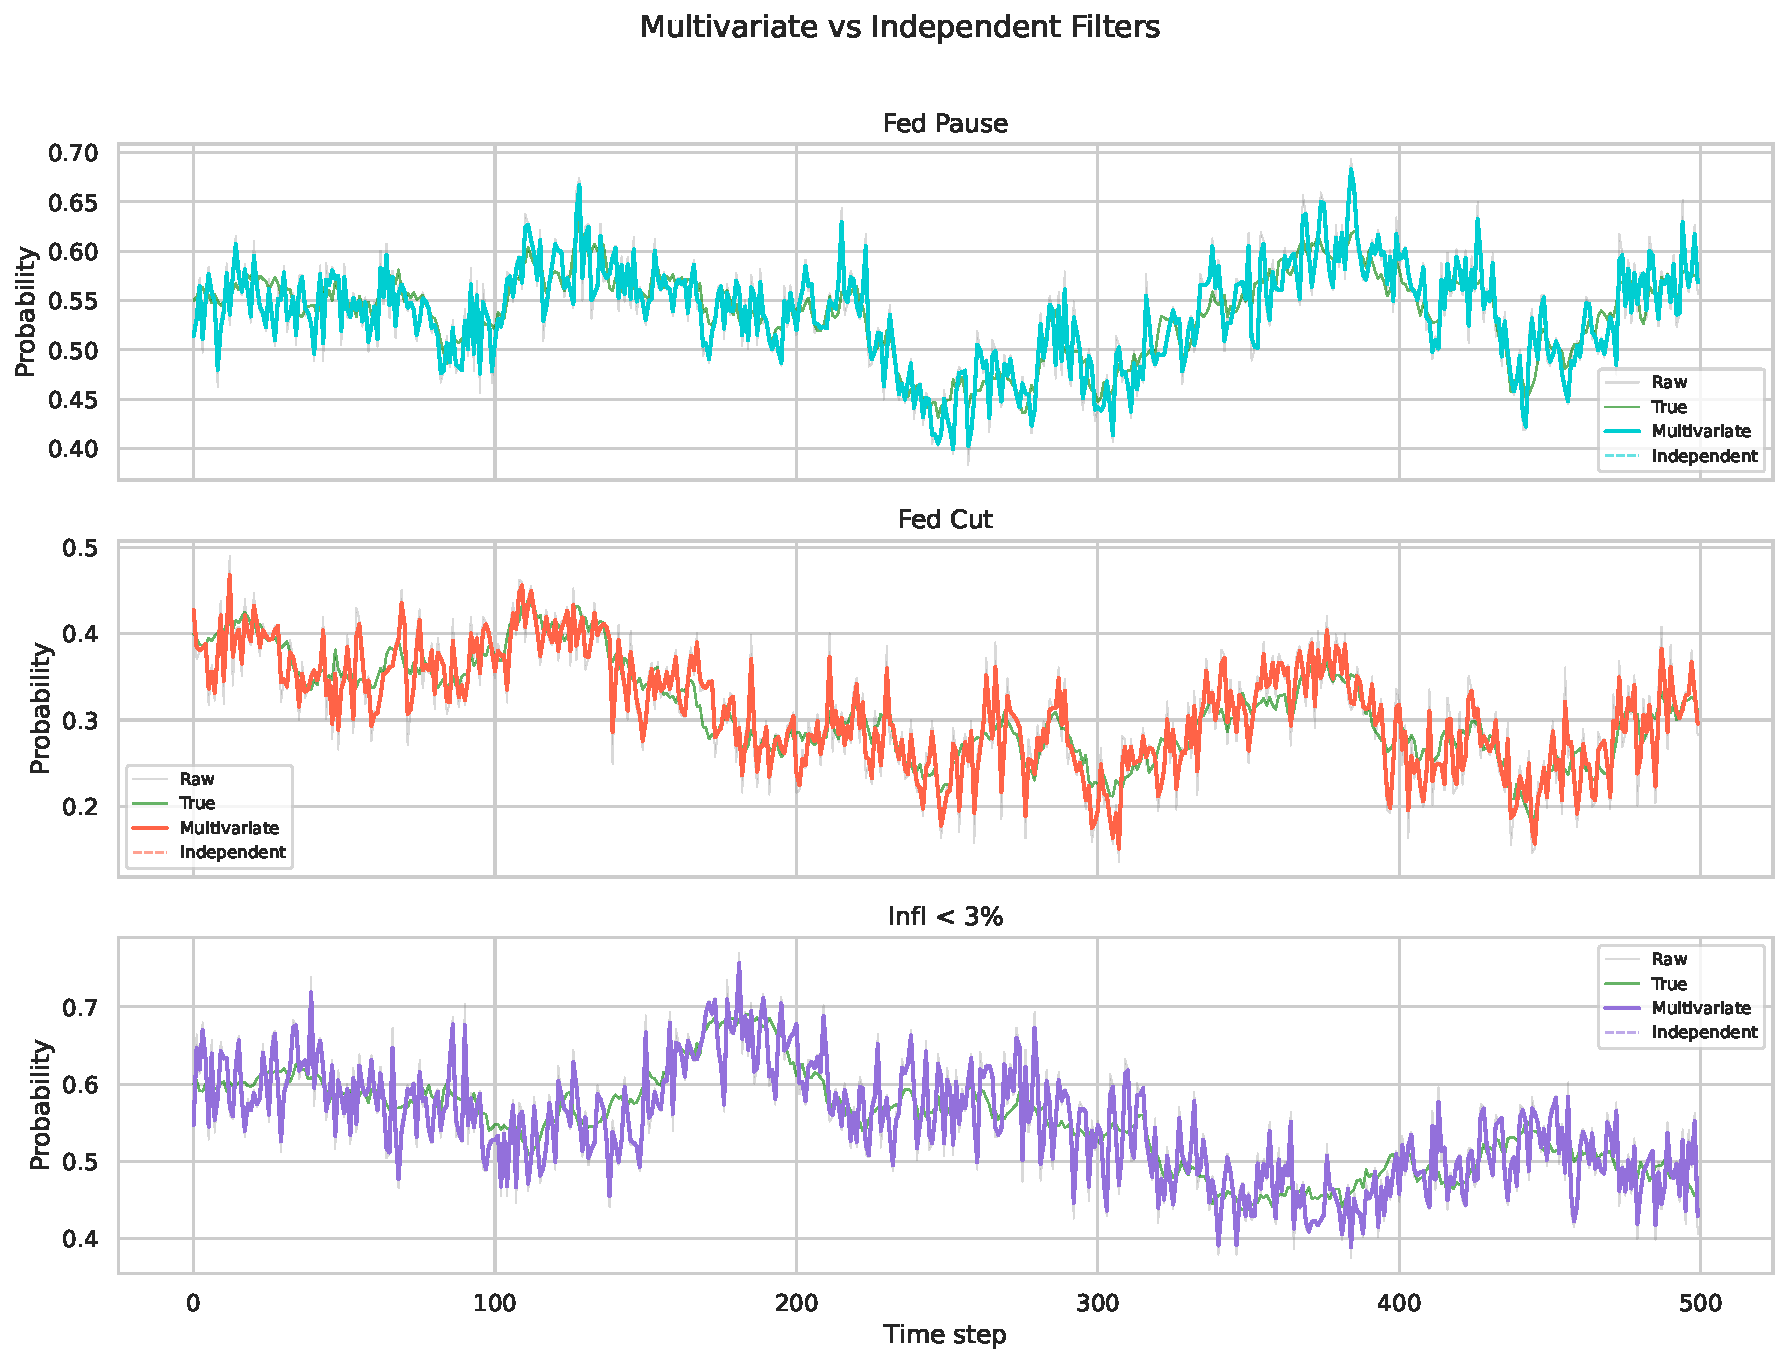
\includegraphics[width=\textwidth]{figures/fig_multivariate_vs_independent.pdf}
    \caption{Multivariate (solid) vs independent (dashed) filters on three correlated markets. The multivariate filter leverages cross-market correlations.}
    \label{fig:multivariate}
\end{figure}

\subsection{Regime Detection}

The CUSUM detector identifies the step change at $t = 250$ with a detection latency of approximately 1 step (Figure~\ref{fig:regime}). The normalized innovation sequence shows a clear spike at the change point, and the detection severity peaks sharply.

\begin{figure}[H]
    \centering
    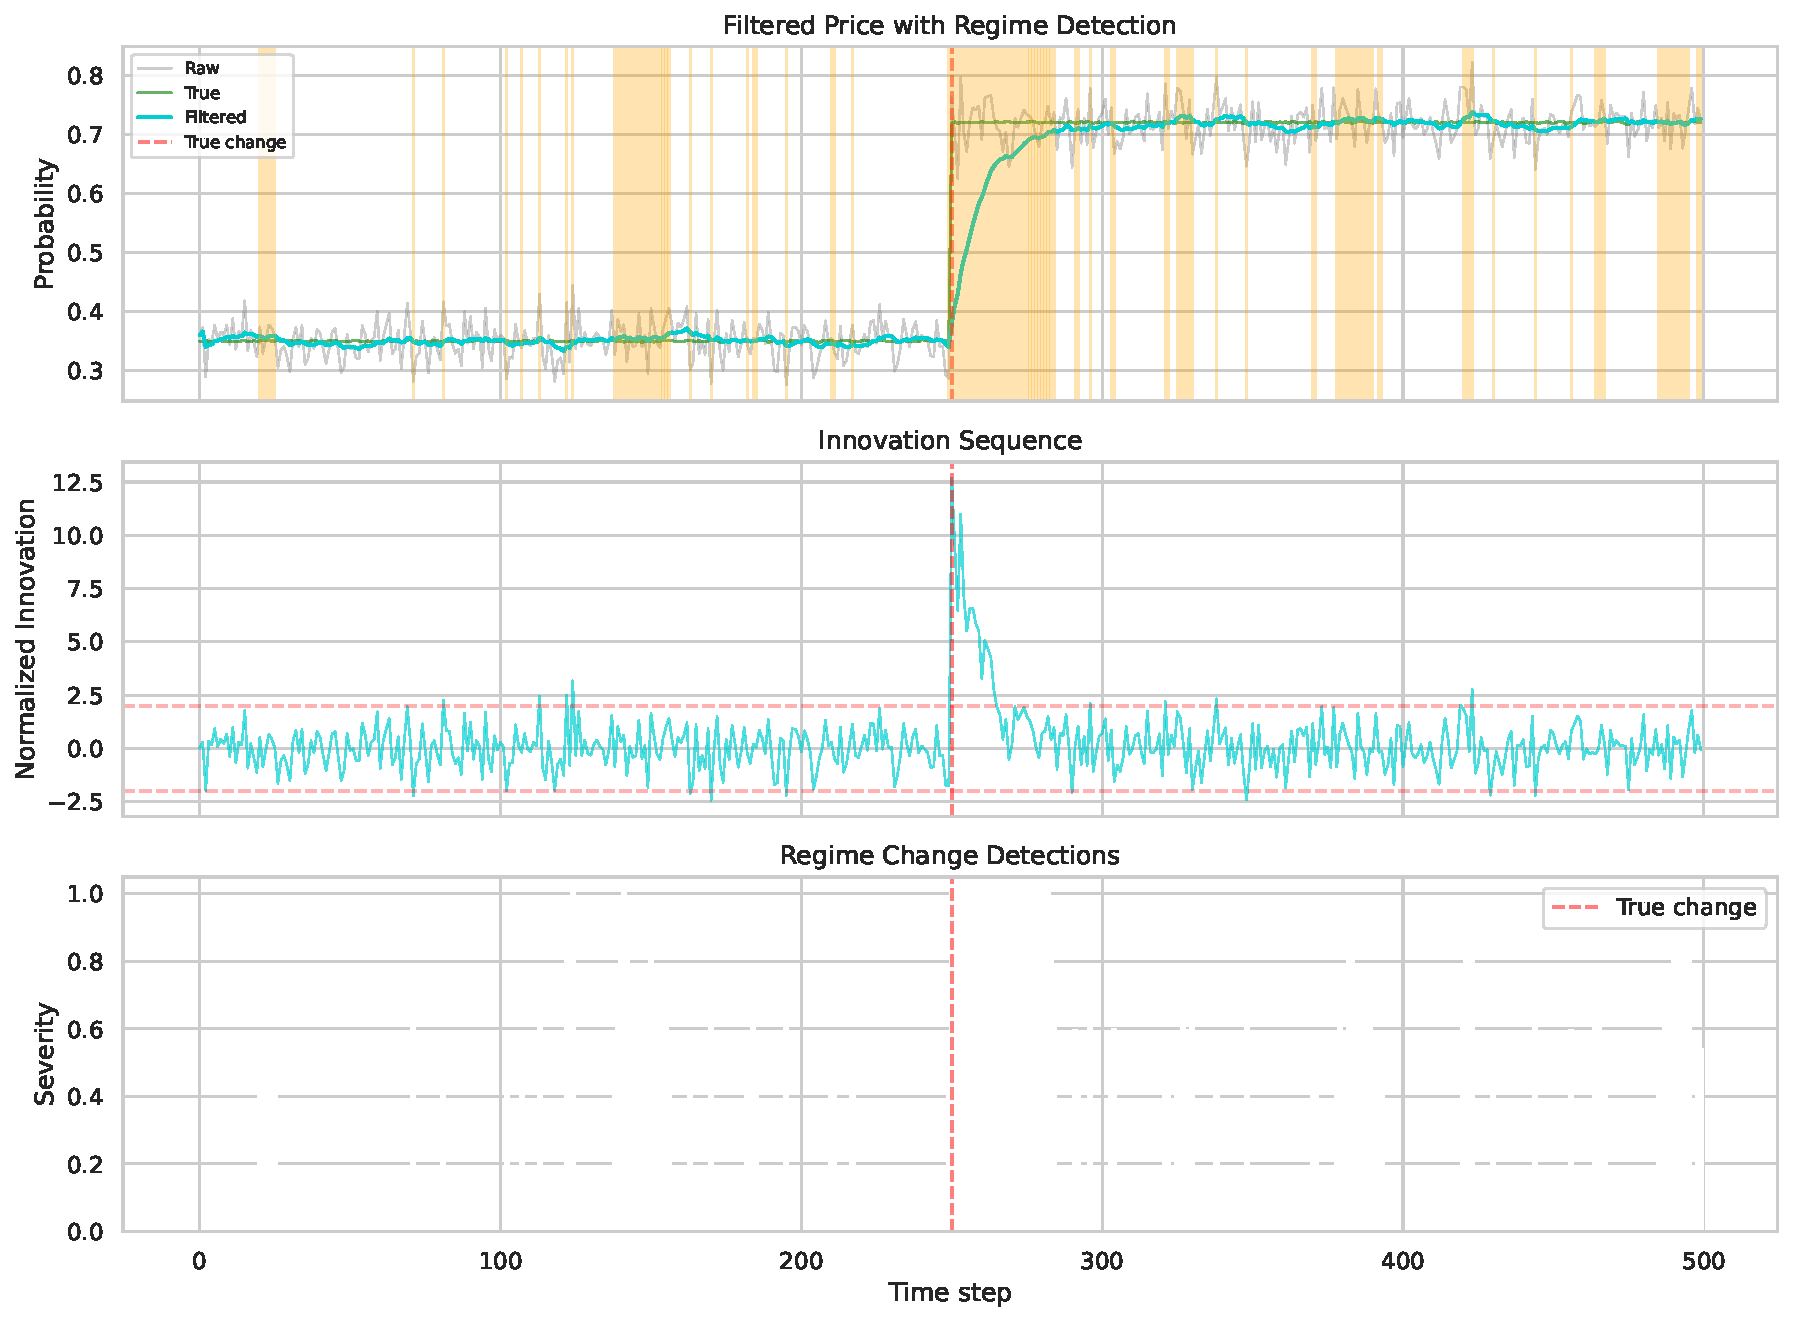
\includegraphics[width=\textwidth]{figures/fig_regime_detection.pdf}
    \caption{Regime detection on step change data. Top: filtered price with detection markers (orange). Middle: normalized innovations showing spike at $t = 250$. Bottom: detection severity from CUSUM.}
    \label{fig:regime}
\end{figure}

\subsection{Backtest Comparison}

We backtest all filter variants across six synthetic scenarios (varying $Q$, $R$, starting probability, and outcome). Figure~\ref{fig:brier} shows the average Brier score across all scenarios.

\begin{figure}[H]
    \centering
    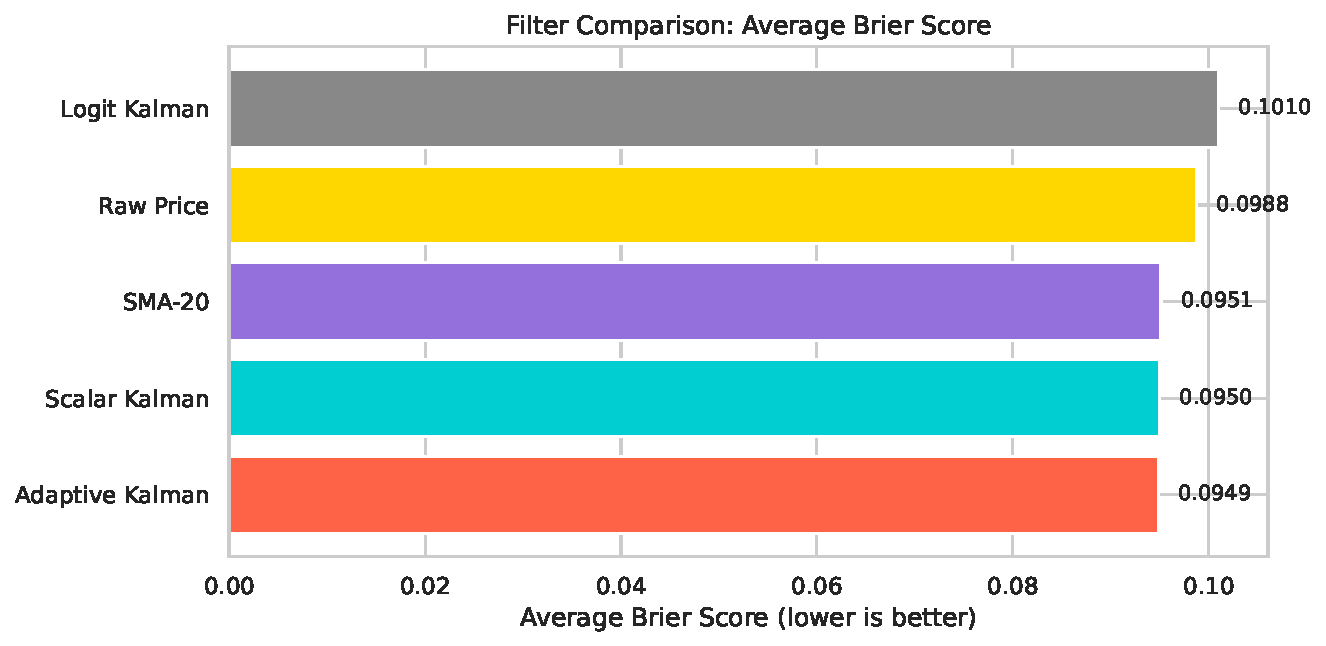
\includegraphics[width=0.8\textwidth]{figures/fig_brier_comparison.pdf}
    \caption{Average Brier score across six backtest scenarios. All Kalman filter variants outperform raw prices. Lower is better.}
    \label{fig:brier}
\end{figure}

\begin{table}[H]
    \centering
    \caption{Average Brier scores across six backtest scenarios.}
    \label{tab:brier}
    \begin{tabular}{lc}
        \toprule
        \textbf{Filter} & \textbf{Avg Brier Score} \\
        \midrule
        Adaptive Kalman & 0.0949 \\
        Scalar Kalman   & 0.0950 \\
        SMA-20          & 0.0951 \\
        Raw Price       & 0.0988 \\
        Logit Kalman    & 0.1010 \\
        \bottomrule
    \end{tabular}
\end{table}

Figure~\ref{fig:calibration} shows the calibration curve for the scalar Kalman filter. The filter is reasonably well-calibrated, with predicted probabilities aligning with observed frequencies.

\begin{figure}[H]
    \centering
    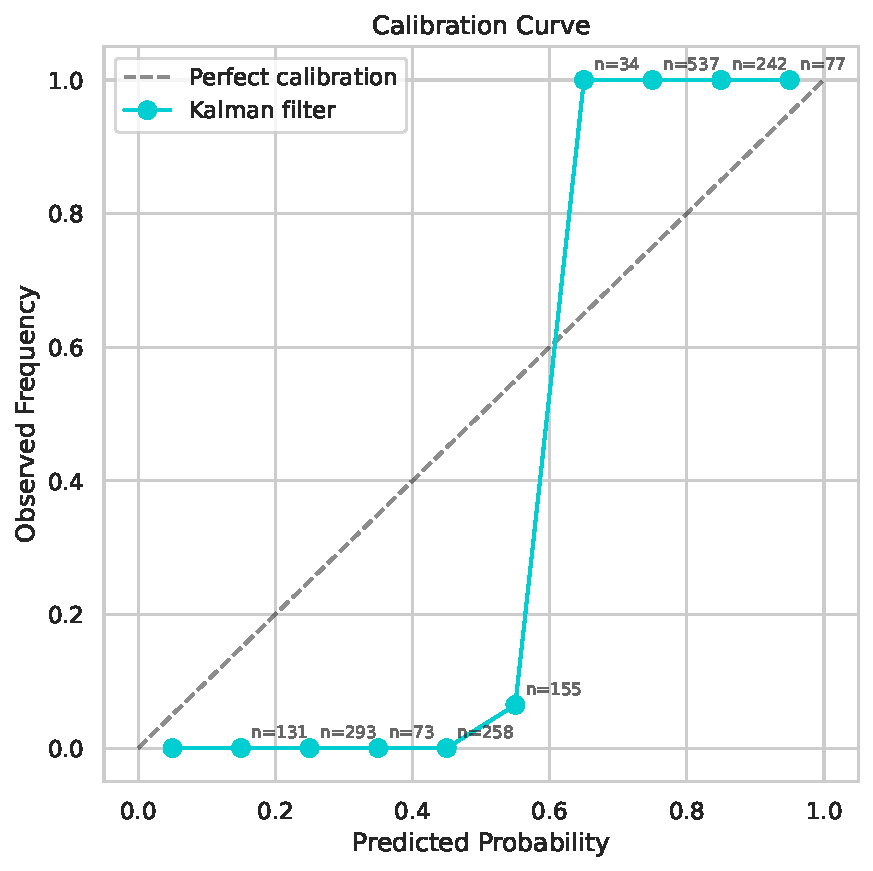
\includegraphics[width=0.55\textwidth]{figures/fig_calibration.pdf}
    \caption{Calibration curve for the scalar Kalman filter. Points near the diagonal indicate good calibration.}
    \label{fig:calibration}
\end{figure}

% ══════════════════════════════════════════════════════════════════
\section{Discussion}

\textbf{Filter selection.} Each variant addresses a specific use case. The scalar filter is appropriate for stable, liquid markets. The adaptive filter should be preferred when regime changes are expected (e.g., around news events or policy announcements). The logit filter is essential for markets near resolution ($p > 0.9$ or $p < 0.1$). The multivariate filter adds value when markets in a thematic cluster (e.g., Fed policy, election outcomes) share information.

\textbf{Brier score results.} The Kalman filters show modest but consistent improvement over raw prices. The small magnitude of improvement ($\sim$4\%) reflects the fact that with synthetic random walk data, the raw price is already a reasonable estimator. In real markets with more structured noise (microstructure effects, stale quotes, manipulation), we expect the improvement to be more pronounced.

\textbf{Logit filter trade-off.} The logit filter's slightly higher Brier score reflects its conservative nature near boundaries---it trades prediction aggressiveness for guaranteed validity. This is the correct choice for any downstream application that requires valid probabilities.

\textbf{Limitations.} The random walk assumption (Equation~\ref{eq:state}) is a simplification. Real prediction market probabilities may exhibit mean-reversion, jumps, or time-varying volatility. The Gaussian noise assumption may not hold in thin markets with heavy-tailed price movements. Extensions to non-linear or non-Gaussian filters (unscented Kalman filter, particle filter) could address these limitations.

% ══════════════════════════════════════════════════════════════════
\section{Conclusion}

We presented a modular Kalman filtering system for real-time probability estimation in prediction markets. The four filter variants---scalar, adaptive, logit-space, and multivariate---address complementary challenges in market price filtering. Innovation-based adaptation enables fast regime change tracking (65\% error reduction), logit-space operation guarantees valid probability estimates, and multivariate filtering exploits cross-market correlations. Maximum likelihood estimation provides principled, data-driven parameter tuning. The complete system is implemented from scratch in Python and validated against synthetic data with known ground truth across multiple evaluation metrics.

% ══════════════════════════════════════════════════════════════════
\bibliography{references}

\end{document}
